\documentclass[8pt]{article}
\usepackage{fancyhdr}
\usepackage{graphicx}
\usepackage{multicol}
\usepackage{capt-of}%%To get the caption
\title{Game-Theoretic Models of Information Overload in Social Networks}
%\author{Krishna Vaidyanathan}
\usepackage[margin=0.7in]{geometry}
\lhead{Krishna Vaidyanathan}
\rhead{February 29, 2016}

\chead{CS 886: Trust and Social Networks}
\pagestyle{fancy}

\newcommand{\bi}{\begin{itemize}}
\newcommand{\ei}{\end{itemize}}

\newcommand{\bn}{\begin{enumerate}}
\newcommand{\en}{\end{enumerate}}

\begin{document}
\centerline{\underline{\textbf{Game-Theoretic Models of Information Overload in Social
        Networks}}}
\paragraph{Authors: } Christian Borgs, Jennifer Chayes, Brian Karrer, Brendan Meeder, R.
Ravi, Ray Reagans, Amin Sayedi

\section{Introduction}
\bi \item Social networks make it convenient to get updates asynchronously.
\item Content of newsfeed becomes important to users.
\item Newsfeed content is based on activity level of user's friends.
\item Thus, newsfeed content is not determined by user.
\item User may be forced to read irrelevant updates.
\ei

\section{Types of Social Networks}
\bn
\item Symmetric: requires consent from both sides to maintain tie - eg.,
    Facebook.
\item Asymmetric: requires consent from only one side to maintain tie - eg.,
    Twitter.
\en
\bi
\item Authors mainly look at asymmetric social networks.
\ei



\section{Assumptions}
\begin{multicols}{2}
\bi
\item Rate of sending updates is key decision variable (see
    Fig~\ref{empirical_evidence}).
\item Updates from friends are useful, but excessive updates have diminishing
    value.
\item Users can be partitioned as producers and consumers of information.
\ei
\columnbreak
\begingroup
%\begin{figure}[H]
%    
    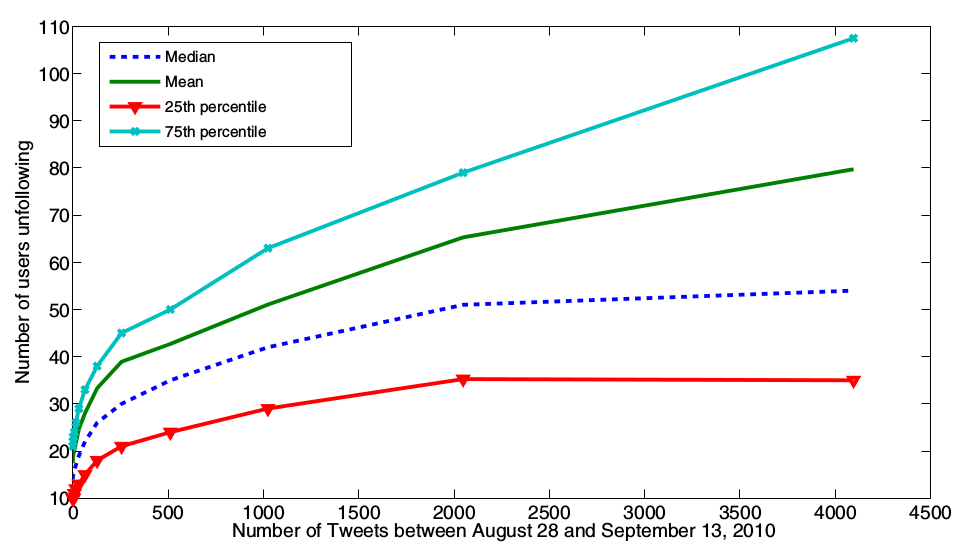
\includegraphics[scale=0.25]{./figures/twitter_data.png}
    \captionof{figure}{Empirical evidence from Twitter data to prove that as rate
       increases number of accounts unfollowing user increases}\label{empirical_evidence}
%\end{figure}
\endgroup
\end{multicols}
\section{Models for Social Networks}
\bi
\item Followership: Users in network will stay in network but unfollow agents
    who give too frequent updates.
\item Engagement: Users get frustrated by high update rate of followees and
    leave the social network.
\ei

\section{Graph Model}
    \bi
\item Complete bipartite graph on two disjoint sets of nodes: producers (C), and
    consumers (F).
\item Edge between producer $i$ and consumer $j$ is associated with a non-negative
    quality score $q_{ij}$.
    \bi
\item $q_{ij}$ denotes utility consumer $j$ derives from producer $i$'s updates.
    \ei
\item Producer $i$ updates at a frequency (rate) of $r_{i}$.
\item Payoff for producer $i$ is $r_i$ times the number of followers he/she has.
    \ei

\section{Followership}
\bi
\item Utility of consumer is $U_{j} = r_{i}q_{ij} - \lambda (\sum_{i}x_i
    r_{i})^2$, where $x_i$ is an indicator variable which is 1 if consumer $j$
    follows producer $i$.
\item Solving for $x_i \in \{0, 1\}$ is hard so simplify to $x_i \in [0,1]$ and greedy model is used.
\item \textbf{Greedy model}: Consider consumer $j$ and let $q_1 \geq \ldots \geq q_n$ be the sorted
    order of $q_{1j},\ldots,q_{nj}$, and $k$ be the largest index such that
    $\sum_{i=1}^{k}r_i \leq q_k$. Under the greedy model, consumer $j$
    follows the $k$ producers for who he has the highest quality and no one
    else.
\item Nash equilibrium not necessarily exists, example where not existing is
    shown.
\item Nash equilibrium exists when consumers follow a global ranking of
    producers.
\item Also when, the dependency graph of a game instance is acyclic. The
    dependency graph is defined for nodes of producers and consumers with a
    directed edge from producer $x$ to producer $y$ if $x$ is valued greater by
    a consumer than $y$.
\item Nash equilibrium can be characterized by a matching from all subsets of
    producers to consumers.
\ei

\section{Engagement}
\bi
\item Nash equilibrium exists for games where all consumers have same degree,
    and when consumers follow one or two celebrities.
\ei

\section{Conclusions}
\subsection{Cons}
\bi
\item Not enough motivation for why particular models of social networks is selected.
\item Matching characterization not elaborated upon.
\item Fractional flow, and greedy model in Followership model not realistic, though understandable why chosen.
\item Might Mixed State Nash equilibrium be looked at?
\ei

\subsection{Pros}
\bi
\item Takes into account rate of update in social networks.
\item Characterization showed in Followership model.
\item Empirical evidence shown for why rate of updates is a valid parameter.
\ei
\end{document}
